%\documentclass[paper=a4,abstract=on,cleardoublepage=empty,numbers=noenddot,toc=bib,12pt,appendixprefix=true]{scrreprt}
\documentclass[%
    a4paper,              % DIN A4
    style=print,          % enables twoside, print colors, and BCOR=15mm
    bibliography=totoc,   % bibliography gets unnumbered entry
    nexus,                % corporate design font
    lnum,                 % use "Versalziffern" instead of "Mediaevalziffern"
    extramargin,          % override corporate design margin to give more space for one-column text
]{tubsbook}

%\usepackage[T1]{fontenc}
\usepackage[utf8]{inputenc}

\usepackage{pgfplots}
%\usepackage{microtype}
\usepackage{xcolor}
    \definecolor{medium-blue}{rgb}{0,0,0.5}
\usepackage{hyperref}
\usepackage{amsmath}
\usepackage{amsthm}
\usepackage{mathtools}
\usepackage[nameinlink]{cleveref}
    \newtheorem{theorem}{Theorem}
    \newtheorem{corollary}{Corollary}
    \theoremstyle{definition}
    \newtheorem{definition}{Definition}
    \newtheorem{lemma}{Lemma}
\usepackage{amsfonts}
\usepackage{todonotes}
\usepackage{tikz}
    \newcommand{\B}{1.36207}

\tikzset{tight/.style={inner sep=1pt}}
\tikzset{bracket/.style={inner sep=10pt,draw=gray,decorate,decoration={brace,amplitude=5pt}}}
\tikzset{filled/.style={fill=black!30!white}}
\tikzset{filled2/.style={fill=black!15!white}}

%\newcommand\hatshape[3][]{
%    \pgfmathsetmacro{\r}{sqrt((#2)/pi)}
%    \pgfmathsetmacro{\s}{sqrt((#3)/pi)}
%
%    \coordinate (top) at (0,{(\r/(sqrt(2)-1)});
%    \coordinate (right) at ({(\r/(sqrt(2)-1)},0);
%    \coordinate (left) at ({(-\r/(sqrt(2)-1)},0);
%
%    \coordinate (leftcenter) at ($({-(\r-\s)/(sqrt(2)-1)},0)+(0,\s)$);
%    \coordinate (leftbottom) at ($(leftcenter)+(-90:\s)$);
%    \coordinate (lefttop) at ($(leftcenter)+(-225:\s)$);
%
%    \coordinate (rightcenter) at ($({(\r-\s)/(sqrt(2)-1)},0)+(0,\s)$);
%    \coordinate (rightbottom) at ($(rightcenter)+(-90:\s)$);
%    \coordinate (righttop) at ($(rightcenter)+(45:\s)$);
%
%    \coordinate (midcenter) at (0,\r);
%
%    \draw[#1] (rightbottom) arc (-90:45:\s) -- (top) -- (lefttop) arc (-225:-90:\s) -- cycle;
%}

\newcommand\hatshape[5][]{
    \pgfmathsetmacro{\r}{sqrt((#2)/pi)}
    \pgfmathsetmacro{\s}{sqrt((#3)/pi)}
    \pgfmathsetmacro{\a}{(#4)}
    \pgfmathsetmacro{\b}{(#5)}

    \coordinate (top) at ({cos((90+(\a-\b)/2))*(\r/cos((\a+\b)/2))},{sin((90+(\a-\b)/2))*(\r/cos((\a+\b)/2)});
    \coordinate (left) at ({-\r/tan(\a/2)},-\r);
    \coordinate (right) at ({\r/tan(\b/2)},-\r);

    \coordinate (leftcenter) at ($(left)+({\s/tan(\a/2)},\s)$);
    \coordinate (leftbottom) at ($(leftcenter)+(-90:\s)$);
    \coordinate (lefttop) at ($(leftcenter)+({-270+\a}:\s)$);

    \coordinate (rightcenter) at ($(right)+({-\s/tan(\b/2)},\s)$);
    \coordinate (rightbottom) at ($(rightcenter)+(-90:\s)$);
    \coordinate (righttop) at ($(rightcenter)+({90-\b}:\s)$);

    \coordinate (topcenter) at ($(top)-({cos((90+(\a-\b)/2))*(\s/cos((\a+\b)/2))},{sin((90+(\a-\b)/2))*(\s/cos((\a+\b)/2)})$);
    \coordinate (topleft) at ($(topcenter)+({-270+\a}:\s)$);
    \coordinate (topright) at ($(topcenter)+({90-\b}:\s)$);

    \coordinate (midcenter) at (0,0);

    %\draw[#1] (right) -- (top) -- (left) -- cycle;
    \draw[#1] (rightbottom) arc (-90:{90-\b}:\s) -- (topright) arc ({90-\b}:{90+\a}:\s) -- (lefttop) arc ({-270+\a}:-90:\s) -- cycle;
}
\newcommand\gemshape[3][]{
    \pgfmathsetmacro{\r}{sqrt((#2)/pi)}
    \pgfmathsetmacro{\s}{sqrt((#3)/pi)}
    \pgfmathsetmacro{\l}{0.85955*sqrt(#3)}
    \pgfmathsetmacro{\ll}{0.7654*\l}
    \pgfmathsetmacro{\a}{45}
    \pgfmathsetmacro{\b}{45}

    \coordinate (top) at ({cos((90+(\a-\b)/2))*(\r/cos((\a+\b)/2))},{sin((90+(\a-\b)/2))*(\r/cos((\a+\b)/2)});
    \coordinate (left) at ({-\r/tan(\a/2)},-\r);
    \coordinate (right) at ({\r/tan(\b/2)},-\r);

    \coordinate (leftcenter) at ($(left)+({\s/tan(\a/2)},\s)$);
    \coordinate (lefttop) at ($(left)+(45:\l)$);
    \coordinate (leftmid) at ($(left)+(22.5:\ll)$);
    \coordinate (leftbottom) at ($(left)+(0:\l)$);

    \coordinate (rightcenter) at ($(right)+({-\s/tan(\b/2)},\s)$);
    \coordinate (righttop) at ($(right)+(135:\l)$);
    \coordinate (rightmid) at ($(right)+(157.5:\ll)$);
    \coordinate (rightbottom) at ($(right)+(180:\l)$);

    %\coordinate (topcenter) at ($(top)-({cos((90+(\a-\b)/2))*(\s/cos((\a+\b)/2))},{sin((90+(\a-\b)/2))*(\s/cos((\a+\b)/2)})$);
    %\coordinate (topleft) at ($(topcenter)+({-270+\a}:\s)$);
    %\coordinate (topright) at ($(topcenter)+({90-\b}:\s)$);

    \coordinate (midcenter) at (0,0);

    \draw[#1] (top) -- (righttop) -- (rightmid) -- (rightbottom) -- (leftbottom) -- (leftmid) -- (lefttop) -- cycle;
    %\draw[#1] (rightbottom) arc (-90:{90-\b}:\s) -- (top) arc ({-270+\a}:-90:\s) -- cycle;
}

\newcommand\hatsinsquare[1]{
    \draw (0,0) rectangle (\B,\B);

    \pgfmathparse{\B-sqrt((1-(#1))/pi)}
    \begin{scope}[shift={(\pgfmathresult,\pgfmathresult)}]
        \begin{scope}[rotate=-45]
            \pgfmathsetmacro{\hata}{1-(#1)}
            \pgfmathsetmacro{\hatb}{1-2*(#1)}
            \hatshape[filled2]{\hata}{\hatb}{45}{45}
            \node at (midcenter) {\hata};
        \end{scope}
    \end{scope}

    \def\comparg{#1}
    \if\comparg0\else
        \pgfmathparse{(sqrt((#1)/pi)}
        \begin{scope}[shift={(\pgfmathresult,\pgfmathresult)}]
            \begin{scope}[rotate=-225]
                \hatshape[filled2]{#1}{0}{45}{45}
                \node at (midcenter) {#1};
            \end{scope}
        \end{scope}
    \fi
}

% alpha, beta, incircle-area of right hat, rounding
\newcommand\hatsinhat[4]{
    \pgfmathsetmacro{\a}{(#1)}
    \pgfmathsetmacro{\b}{(#2)}
    \pgfmathsetmacro{\x}{(#3)}
    \pgfmathsetmacro{\round}{(#4)}
    \pgfmathsetmacro{\f}{(cos(\b/2)^2*sec(\a/2+\b/2)^2*(1-sin(\a)))}
    \pgfmathsetmacro{\g}{(cos(\a/2)^2*sec(\a/2+\b/2)^2*(1-sin(\b)))}

    \hatshape{1}{\round}{\a}{\b}

    \def\comparg{\x}
    \if\comparg0\else
        \pgfmathparse{sqrt(1/pi)/tan(\b/2)-sqrt(((\x))/pi)/tan(\b/2)}
        \begin{scope}[shift={(\pgfmathresult,0)}]
            \pgfmathparse{sqrt(1/pi)-sqrt(\x/pi)}
            \begin{scope}[shift={(0,-\pgfmathresult)}]
                \pgfmathsetmacro{\hata}{\x}
                \pgfmathsetmacro{\hatb}{max(\round,\x-\g*(1-\x)/(\f)))}
                \hatshape[filled2]{\hata}{\hatb}{90}{\b}
                \node at (midcenter) {\hata};
            \end{scope}
        \end{scope}
    \fi

    \def\comparg{\x}
    \if\comparg1\else
        \pgfmathparse{sqrt(1/pi)/tan(\a/2)-sqrt(((1-\x))/pi)/tan(\a/2)}
        \begin{scope}[shift={(-\pgfmathresult,0)}]
            \pgfmathparse{sqrt(1/pi)-sqrt((1-\x)/pi)}
            \begin{scope}[shift={(0,-\pgfmathresult)}]
                \pgfmathsetmacro{\hata}{1-\x}
                \pgfmathsetmacro{\hatb}{\round}
                \pgfmathsetmacro{\hatb}{max(\round,(1-\x)-\f*(\x)/(\g)))}
                \hatshape[filled2]{\hata}{\hatb}{\a}{90}
                \node at (midcenter) {\hata};
            \end{scope}
        \end{scope}
    \fi
}

% incircle-area of right hat, rounding
\newcommand\gemsingem[2]{
    \pgfmathsetmacro{\a}{45}
    \pgfmathsetmacro{\b}{45}
    \pgfmathsetmacro{\x}{(#1)}
    \pgfmathsetmacro{\round}{(#2)}
    \pgfmathsetmacro{\f}{(cos(\b/2)^2*sec(\a/2+\b/2)^2*(1-sin(\a)))}
    \pgfmathsetmacro{\g}{(cos(\a/2)^2*sec(\a/2+\b/2)^2*(1-sin(\b)))}

    \gemshape{1}{\round}

    \def\comparg{\x}
    \if\comparg0\else
        \pgfmathparse{sqrt(1/pi)/tan(\b/2)-sqrt(((\x))/pi)/tan(\b/2)}
        \begin{scope}[shift={(\pgfmathresult,0)}]
            \pgfmathparse{sqrt(1/pi)-sqrt(\x/pi)}
            \begin{scope}[shift={(0,-\pgfmathresult)},rotate=135]
                \pgfmathsetmacro{\hata}{\x}
                \pgfmathsetmacro{\hatb}{max(\round,\x-\g*(1-\x)/(\f)))}
                \gemshape[filled2]{\hata}{\hatb}
                \node at (midcenter) {\hata};
            \end{scope}
        \end{scope}
    \fi

    \def\comparg{\x}
    \if\comparg1\else
        \pgfmathparse{sqrt(1/pi)/tan(\a/2)-sqrt(((1-\x))/pi)/tan(\a/2)}
        \begin{scope}[shift={(-\pgfmathresult,0)}]
            \pgfmathparse{sqrt(1/pi)-sqrt((1-\x)/pi)}
            \begin{scope}[shift={(0,-\pgfmathresult)}]
                \pgfmathparse{\x < 0.1715 ? 0 : -135}
                \begin{scope}[rotate=\pgfmathresult]
                    \pgfmathsetmacro{\hata}{1-\x}
                    \pgfmathsetmacro{\hatb}{\round}
                    \pgfmathsetmacro{\hatb}{\x < 1/3 ? (1-\x) : max(\round,(1-\x)-\f*(\x)/(\g))}
                    \pgfmathsetmacro{\fillstyle}{\x < 1/3 ? "filled" : "filled2"}
                    \gemshape[\fillstyle]{\hata}{\hatb}
                    \node at (midcenter) {\hata};
                \end{scope}
            \end{scope}
        \end{scope}
    \fi
}

\newcommand\hatconstruction{
    \hatshape[draw=none]{1}{0.3}

    \draw[dashed] (rightcenter) circle(\s);
    \draw[dashed] (leftcenter) circle(\s);
    \draw[dashed] (midcenter) circle(\r);
    \draw[dashed] (right) -- (top) -- (left) -- cycle;

    \draw[tight] (rightcenter) -- node[below left] {$s$} ++(-45:\s) -- node[below right] {$s$} ++(45:\s) coordinate (rightright) {} -- node[right] {$s$} ++(-90:\s) -- node[above] {$s$} (right);
    \draw[thick,orange] (rightright) -- node[sloped,above] {$s\sqrt{2}$} (right);

    \draw[tight] (leftcenter) -- node[above] {$s$} ++(180:\s) -- node[left] {$s$} ++(-90:\s) coordinate (leftleft) {} -- node[below left] {$s$} ++(135:\s) -- node[below right] {$s$} (left);
    \draw[thick,orange] (leftleft) -- node[below] {$s\sqrt{2}$} (left);

    \draw[thick,left,blue] (0,0) -- node {$r$} (midcenter) -- node {$r\sqrt{2}$} (top);
    \draw (midcenter) -- node[below right] {$r$} +(45:\r) -- node[above right] {$r$} (top);
    \draw[thick,red] (left) -- node[sloped,above] {$(r+r\sqrt{2})\sqrt{2}$} (top);

    \coordinate (leftofleft) at ($(left)+(180:5pt)$);
    \coordinate (belowleft) at ($(left)-(90:5pt)$);
    \coordinate (farbelowleft) at ($(left)-(90:10pt)$);
    \coordinate (abovetop) at ($(top)+(45:5pt)$);
    \coordinate (farabovetop) at ($(top)+(45:10pt)$);
    \coordinate (faraboveright) at ($(right)+(45:10pt)$);
    \coordinate (aboverightright) at ($(rightright)+(45:5pt)$);
    \coordinate (leftend) at ($(leftleft)-(90:5pt)$);
    \coordinate (rightend) at ($(rightright)-(90:5pt)$);
    \coordinate (totheright) at ($(rightcenter)+(0:\s)$);
    \coordinate (rightend) at ($(totheright)-(90:5pt)$);

    \draw[bracket] (leftofleft) -- node[left] {$h(a)$} (leftofleft |- top);
    \draw[bracket] (rightend |- belowleft) -- node[below] {$w(a,b)$} (leftend |- belowleft);
    \draw[bracket] (rightend |- farbelowleft) -- node[below] {$w'(a,b)$} (left |- farbelowleft);
    \draw[bracket] (abovetop) -- node[above,sloped] {$d(a,b)$} (aboverightright);
    \draw[bracket] (farabovetop) -- node[above,sloped] {$d'(a)$} (faraboveright);
}

    \usetikzlibrary{calc}
    \usetikzlibrary{arrows}
\usepackage{graphicx}
    \graphicspath{{images/}}
\usepackage{algorithm}
\usepackage{algpseudocode}
    \renewcommand{\algorithmicrequire}{\textbf{Input:}}
    \renewcommand{\algorithmicensure}{\textbf{Output:}}
\usepackage{chngcntr}
    \counterwithout{equation}{chapter}

\newcommand{\C}{\mathbb{C}}
\newcommand{\s}{\sqrt{2}}
\DeclareMathOperator{\mysum}{sum}
\DeclareMathOperator*{\argmin}{arg\,min}


\usepackage[english]{babel} % hyphenation

\hypersetup{
    colorlinks, linkcolor={medium-blue},
    citecolor={medium-blue}, urlcolor={medium-blue}
}

%\titlehead{
%    \begin{center}
%        \includegraphics[width=0.5\textwidth]{square_example.png}
%    \end{center}
%}

\subject{Master's Thesis}
\title{Algorithms\\for Circle Packing}
\author{\sffamily\LARGE Sebastian Morr}
\date{\large June 2, 2016}
\publishers{\textbf{Institute of Operating Systems and Computer Networks\\Prof.\,Dr.\,Sándor Fekete}\\
\vspace*{2em}
Supervisor:\\
Super\,Visor,\,M.\,Sc.}

\begin{document}
\frontmatter % roman page numbering

\maketitle
\cleardoublepage

% statement of originality
\thispagestyle{plain} % no header
\vspace*{7cm}
\centerline{\bfseries Statement of Originality}
\vspace*{1em}
\noindent
This thesis has been performed independently with the support of my supervisors.
To the best of the author's knowledge, this thesis contains no material previously
published or written by another person except where due reference is made in the text.

\par
  \bigskip\noindent Braunschweig, \today \par
  \vspace*{10mm}
  \hfill\hrulefill
\cleardoublepage

% abstract
\thispagestyle{plain} % no header
\centerline{\bfseries Abstract}
\vspace*{1em}
\noindent
Very abstract indeed.
\cleardoublepage

% include Aufgabenstellung pdf
%\includepdf[pages=-]{aufgabenstellung/Aufgabenstellung}
%\cleardoublepage

\section*{Acknowledgments}

I would like to thank the following people for their support in the creation of this thesis:

\section*{Colophon}

This document was created using \LaTeXe\ by Leslie Lamport and contributors, and \KOMAScript\ by Frank Neukam, Markus Kohm, and Axel Kielhorn. The figures were created using PGFPlots by Christian Feuersänger and Ti\textit{k}Z by Till Tantau, the key combinations were produced with \emph{menukeys} by Tobias Weh. The text is set in the Latin Modern font family by Bogusław Jackowski, Janusz M. Nowacki and Marcin Woliński, the monospaced font is \texttt{Bera Mono}, based on Bitstream Vera.

\cleardoublepage
\setcounter{tocdepth}{2}

\tableofcontents
\cleardoublepage

%\listoffigures
%\cleardoublepage
%
%\listoftables
%\cleardoublepage

\mainmatter % arabic numbering

\chapter{Introduction}

\begin{figure}[htb]
    \centering

    \begin{tikzpicture}[scale=2.5]
        \squareworstcase
    \end{tikzpicture}

    \caption{Worst-case instance for packing density?}
    \label{fig:worst-case}
\end{figure}

Consider the circle packing shown in \Cref{fig:worst-case}. For these two circles, the surrounding square is the smallest one in which the circles can be packed. We considered the following problem: Does this instance constitute the worst case in terms of packing density? Put differently, can all other sets of circles with the same combined area as these two
%(like the one in \Cref{fig:big-question})
be packed into this specific square?
We will give a constructive proof that this is indeed the case.

\begin{figure}[htb]
    \centering

    \begin{tikzpicture}[scale=2.5]
        \bigquestion
    \end{tikzpicture}

    \caption{Can these circles be packed?}
    \label{fig:big-question}
\end{figure}

\chapter{Preliminaries}

\section{Circle instances}

We start off with some definitions which make our life easier when talking about circles and circle instances:

\begin{definition}
    For each $0 \le a$, an \emph{$a$-circle} is a circle with an area of $a$.
\end{definition}

\begin{definition}
    A \emph{circle instance} is a multiset of non-negative real numbers, which define the circles' areas.
\end{definition}

\begin{definition}
    For a circle instance $A$, $\mysum(A)$ is the combined area of the instance's circles.
\end{definition}

\begin{definition}
    $\C$ is the set of all circle instances. $\C(a)$ consist of exactly those circle instances with a combined area of at most $a$. Finally, $\C(a,b)$ consists of exactly those circle instances $A \in \C(a)$, for which each circle in $A$ has an area of at least $b$.
\end{definition}

\begin{lemma}
    If the circle instance shown in \Cref{fig:b} has a combined area of $a$, the square has an area of $\frac{3+2\s}{\pi}a \approx 1.85525a$. Call this worst-case factor $\Psi$.
\end{lemma}

\begin{proof}
    Note that because a circle of radius $r$ has an area of $a = \pi r^2$, an $a$-circle has a radius of $r = \sqrt{\frac a \pi}$. Then, by construction as seen in \Cref{fig:b}:

    $$\Psi a = \left(2r + 2\frac{r}{\s}\right)^2 = r^2\left(2+\s\right)^2 = \frac{\frac a 2}{\pi}\left(4+4\s+2\right) = \frac{3+2\s}{\pi}a$$
\end{proof}

\begin{figure}[htb]
    \centering

    \begin{tikzpicture}[scale=3]
        \squareworstcaseconstruction
    \end{tikzpicture}

    \caption{Constructing $\Psi$.}
    \label{fig:b}
\end{figure}

Our problem can now be expressed like this: Can all circle instances $A \in \C(a)$ be packed into a square with an area of $\Psi a$? This will be \Cref{th:circlesinsquare}, and the rest of this paper will build up to its proof.

\chapter{Common techniques}

\section{Greedy splitting}

The core idea of the proposed packing algorithms is to repeatedly split the set of input circles into groups. The method which performs this splitting resembles a greedy scheduling algorithm. It is going to be important for the packing algorithm that the ratio of the groups' sizes is close to certain factors.

\textsc{Split} takes two parameters: The first is an arbitrary circle instance $C$. The second is a tuple of positive factors, which determines which percentages of $C$'s total area should go into the respective groups. For example, if we wanted to split $C$ into half, we would choose the tuple $(1,1$).
It will not always be possible to achieve this desired ratio, but we can derive some properties from the resulting subinstances if their sizes derive from this factor.

\begin{algorithmic}
    \Require A circle instance $C$ and a tuple of positive numbers $F = (f_0, f_1, \dots, f_n)$
    \Ensure Circle instances $C_1, C_2, \dots, C_n$
    \Function{Split}{$C,F$}
        \For{$i = 1$ to $n$}
            \State $C_i \gets \emptyset$
        \EndFor
        \State Sort $C$ descending by size
        \ForAll{$c \in C$}
            \State $j = \min_{1 \le i \le n} \frac{\mysum(C_i)}{f_i}$\Comment{Find the index of the emptiest instance}
            \State $C_j \gets C_j \cup \{c\}$
        \EndFor
    \EndFunction
\end{algorithmic}

\begin{theorem}\label{th:split-property}
    \textsc{Split}$(C,F)$ decomposes $C \in \C$ into $n$ circle instances with $C_0 + C_1 + \dots + C_n = C$.

    Define $r_i = \frac{\mysum(C_i)}{f_i}$ as the relative filling level of $C_i$.
    Set $r^* = \min\{r_0,r_1,\dots,r_n\}$.
    Then all $c \in C_i$ have a size of at least $f_i(r_i-r^*)$.
\end{theorem}

\begin{proof}
    Assume for contradicion $C_i$ contained an element smaller than $f_i(r_i-r^*)$. All elements which were put into $C_i$ after that have to be at least as small, as the elements were sorted by descending size. So the last element put into $C_i$ (let us call it $c$) would be smaller than $f_i(r_i-r^*)$, as well.
    But this means that $\frac{\mysum(C_i) - c}{f_i} > \frac{\mysum(C_i) - f_i(r_i-r^*)}{f_i} = r_i - (r_i-r^*) = r^*$, meaning that at the moment $c$ was inserted, the relative filling level of $C_i$ would already have been larger than $r^*$, a contradiction to the algorithm's greedy nature, as \textsc{Split} would have put the element into a less filled instance in this situation.
\end{proof}

\section{Shapes}

\begin{definition}
    For any $C \subseteq \C$, a $C$-shape is a shape in which each $c \in C$ can be packed.
\end{definition}

For example, if a shape is a $\C(a)$-shape, each circle instance with a total area of $a$ can be packed into the shape.

\begin{theorem}
    A shape is a $\mathcal{C}$-shape, if, for a given decomposition method, for all possible decompositions $C_1, C_2, \dots, C_n$ of any $C \in \mathcal{C}$, one can always find $n$ shapes in which the resulting subinstances can be packed, and which fit into the original shape.
\end{theorem}

\begin{definition}\label{def:tangled}
    For any tuple of positive numbers $F$, we say that $n$ shapes are $F$-tangled, if the $i$-th shape is a $\C(a_i, a_i - f_i r^*)$-shape, with $r^* = min\{\frac{a_i}{f_i}|i \in 1,2,\dots,n\}$.
\end{definition}

\begin{theorem}
    A shape is a $\C(a,b)$-shape, if there is a tuple of positive numbers $F$, so that for all $a_1 + a_2 + \dots + a_n \le a$, one can find a $\C(a_1)$-shape, a $\C(a_2)$-shape, \dots, and a $\C(a_n)$-shape, which are $F$-tangled and fit into the original shape.
\end{theorem}

\begin{theorem}\label{th:split-tangle}
    Given an arbitrary $C \in \C(a,b)$ and a tuple of positive numbers $F$, use \textsc{Split}$(C,F)$ to decompose $C$ into $n$ subinstances. Call the subinstances' totals $a_1$, $a_2$, \dots, $a_n$. If we find $n$ shapes, each of which is a $\C(a_i)$-shape, and these shapes are $F$-tangled, we can pack $C$ into the shapes.
\end{theorem}

\begin{proof}
    By \Cref{th:split-property}, \textsc{Split} only produces subinstance $C_i \in \C(a_i, (a_i, a_i-f_i r^*))$.
    As our shapes are $F$-tangled, by \cref{def:tangled}, the $i$-th shape is a $\C(a_i, (a_i, a_i - f_i r^*))$-shape, so the $i$-th subinstance can be packed.
\end{proof}

\begin{theorem}
    For a given shape, if there is an $F$ so that for all $a_1 + a_2 + \dots + a_n \le a$ one can find $F$-tangled $\C(a_i, b)$-shapes which can be packed into the original shape, that shape is a $\C(a,b)$-shape.
\end{theorem}

\begin{proof}
    Given an arbitrary $C \in \C(a,b)$, regardless of which totals \textsc{Split} produces, we know from \cref{th:split-tangle} that we can always pack them into our $F$-tangled shapes. As these shapes also fit into the original shape, we know that we can pack $C$ into that shape.
\end{proof}

\chapter{Hats}

The packing algorithm will also involve a specific family of shapes, which can recursively be packed into each other. We call these shapes \emph{hats}:

\begin{definition}
    For each $0 \le b \le a$, an ($a,b$)-hat is a triangle with an incircle of area $a$, whose corners are rounded to the radius of a $b$-circle (see \Cref{fig:hat}).
    An $a$-hat is an $(a,0)$-hat.
    If we say \emph{obtuse hat}, \emph{right hat}, or \emph{acute hat}, the hat is based on an obtuse/right/acute triangle.
\end{definition}

\begin{figure}[htb]
    \centering

    \begin{tikzpicture}[scale=3]
        \hatsimple
    \end{tikzpicture}

    \caption{An $(a,b)$-hat.}
    \label{fig:hat}
\end{figure}

%%For the following proofs, we need to know a hat's dimensions in detail. We construct these measures using \Cref{fig:construction}.
%%
%%\begin{lemma}\label{lm:sizes}
%%    Let $r$ be the radius of an $a$-circle, and $s$ be the radius of a $b$-circle.
%%
%%    A ($a,b$)-hat has
%%    \begin{itemize}
%%        \item height $h(a) = \textcolor{blue}{r + r\s} = \sqrt{\frac a \pi}(1+\s)$,
%%        \item width $w(a,b) = 2\textcolor{blue}{(r+r\s)} - 2\textcolor{orange}{s\s} = \sqrt{\frac a \pi}(2+2\s)-\sqrt{\frac b \pi}2\s$,
%%        \item and diagonal $d(a,b) = \textcolor{red}{(r+r\s)\s} - \textcolor{orange}{s\s} = \sqrt{\frac a \pi}(2+\s)-\sqrt{\frac b \pi}\s$.
%%    \end{itemize}
%%
%%    We define two additional measures for the case when one of the corners is not rounded:
%%    \begin{itemize}
%%        \item corner-width $w'(a,b) = w(a,b) + \textcolor{orange}{s\s} = \sqrt{\frac a \pi}(2+2\s)-\sqrt{\frac b \pi}\s$,
%%        \item and corner-diagonal $d'(a) = d(a,0) = \sqrt{\frac a \pi}(2+\s)$.
%%    \end{itemize}
%%\end{lemma}
%%
%%\begin{figure}[tb]
%%    \centering
%%
%%    \begin{tikzpicture}[scale=4]
%%        \hatconstruction
%%    \end{tikzpicture}
%%
%%    \caption{Constructing the dimensions of an $(a,b)$-hat.}
%%    \label{fig:construction}
%%\end{figure}
%%
\begin{figure}[tb]
    \centering

    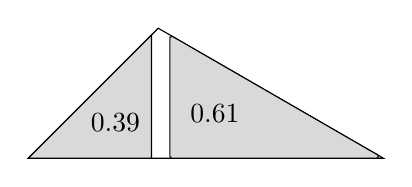
\begin{tikzpicture}[scale=1.3]
        \hatsinhat{45}{30}{0.61}{0}
    \end{tikzpicture}
    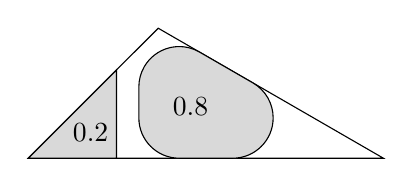
\begin{tikzpicture}[scale=1.3]
        \hatsinhat{45}{30}{0.8}{0}
    \end{tikzpicture}
    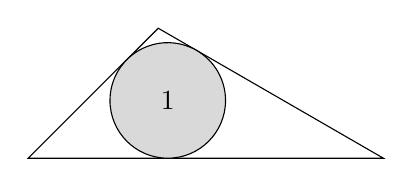
\begin{tikzpicture}[scale=1.3]
        \hatsinhat{45}{30}{1}{0}
    \end{tikzpicture}

    \caption{Hat-in-hat packings for different values of $x$}
    \label{fig:hatsinhat}
\end{figure}

\begin{lemma}\label{th:hatsinhat}
    For each $a$-hat with smaller angles $\alpha$ and $\beta$,
    for $$f = \frac{1}{1+\frac{1+\cot(\frac{\pi}{4}-\frac{\alpha}{2}))^2}{(1+\cot(\frac{\pi}{4}-\frac{\beta}{2}))^2}}$$,
    any $(f,1-f)$-tangled right hats with an incircle sum of less than $a$ can be packed into the $a$-hat.
\end{lemma}

\begin{proof}
    Place the hats' tips at the bottom of the $a$-hat and push them as far to the left/right as possible, like in \Cref{fig:hatsinhat}.

    This placement constitutes a valid packing if (1) the hats do not overlap each other and (2) the hats fit into the $a$-hat individually.
    \begin{itemize}
        \item[(1)]
            \begin{figure}[tb]
                \centering

                \begin{tikzpicture}[scale=3]
                    \hatlr{60}{30}{51}{25}
                \end{tikzpicture}

                \caption{$l^2 + r^2 \le 1$ holds for each non-acute triangle}
                \label{fig:hatlr}
            \end{figure}

            We first normalize the container hat's width to 1 and make an observation about the partial widths $l$ and $r$ in \cref{fig:hatlr}: If the top angle is a right angle, the partial widths have the same lengths as the triangle's two cathetus $x$ and $y$, so $l^2 + r^2 = 1$. If the top angle is obtuse, but the incircle's center stays at the same $x$-coordinate (like the dotted variant), both $l$ and $r$ shrink, so for each hat, $l^2 + r^2 \le 1$.

            \begin{figure}[tb]
                \centering

                \begin{tikzpicture}[scale=3]
                    \hatsoverlap{45}{30}{0.7}{0}
                \end{tikzpicture}

                \caption{$f^2 + g^2 = 1$ for each non-acute triangle}
                \label{fig:hatsoverlap}
            \end{figure}

            We then observe that the hats to be packed don't overlap if their incircles don't overlap, which is true if in \cref{fig:hatsoverlap}, $lf + rg \le 1$ holds. Also note that for \emph{similar} hats, the ratio between their incircle's area and the square of their widths is constant. This means that if $a_1 + a_2 = a$, $f^2 + g^2 = 1$. Thus:

            \begin{align*}
                lf + rg
                &\le lf + \sqrt{1-l^2} \sqrt{1-f^2}\\
                &= lf + \sqrt{(1-l^2)(1-f^2)}\\
                &= lf + \sqrt{1 - f^2 - l^2 + l^2f^2}\\
                &\le lf + \sqrt{1 - 2lf + l^2f^2}\tag{\theequation}\label{eq:am-gm}\\
                &= lf + \sqrt{(1-lf)^2}\\
                &= 1
            \end{align*}

            Line \ref{eq:am-gm} is a consequence of the inequality of arithmetic and geometric means.

        \item[(2)]
            The hats fit into the $a$-hat individually if their corner-width never gets larger than the $(x+y)$-hat's diagonal, $d(x+y,0)$.
            \Cref{lm:sizes} directly tells us that the $x$-hat has a corner-width of at most
            \begin{align*}
                w'(x,0) \le w'(\frac{x+y}{2},0) = \sqrt{\frac{\frac{1}{2}}{\pi}}(2+2\s) + 0 = d(x+y,0)
            \end{align*}

            For the $(y,y-x)$-hat, we can show that $w'(y,y-x) \le d(x+y,0)$: \todo[inline]{algebraic proof TBD :-)}

            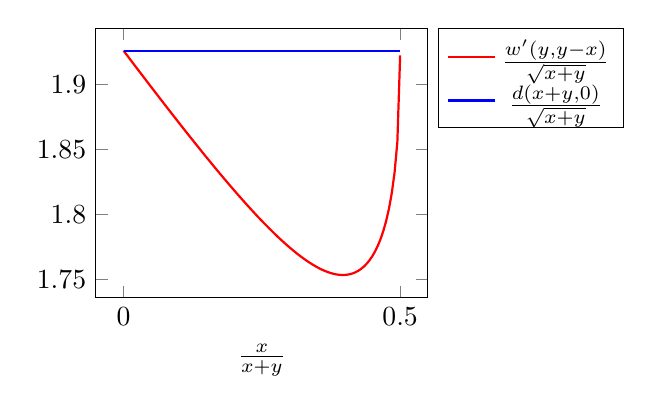
\begin{tikzpicture}
                \begin{axis}[height=5cm,xtick={0,0.5},xlabel=$\frac{x}{x+y}$,domain=0:0.5,legend pos=outer north east,no markers,samples=100]
                    \addplot[red,thick] {sqrt((1-x)/pi)*(2+2*sqrt(2))-sqrt((1-2*x)/pi)*sqrt(2)};
                    \addplot[blue,thick] {sqrt(1/pi)*(2+sqrt(2))};
                    \legend{$\frac{w'{(y,y-x)}}{\sqrt{x+y}}$,$\frac{d{(x+y,0)}}{\sqrt{x+y}}$}
                \end{axis} 
            \end{tikzpicture}
    \end{itemize}
\end{proof}
%
%\begin{theorem}\label{th:roundedhatsinhat}
%    For any $0 \le b \le x \le y$, an $(x,b)$-hat and an $(y,\max(y-x,b))$-hat can always be packed in an $(x+y,b)$-hat.
%\end{theorem}
%
%\begin{proof}
%    The container's lower corners are now rounded to the radius of a $b$-circle, and we need to show that the two hats still fit inside. But the two corners placed in the container's corners are also rounded to (at least) the same radius, so they will never overlap the container, see \Cref{fig:rounding-hats}.
%\end{proof}
%
\begin{figure}[htb]
    \centering

    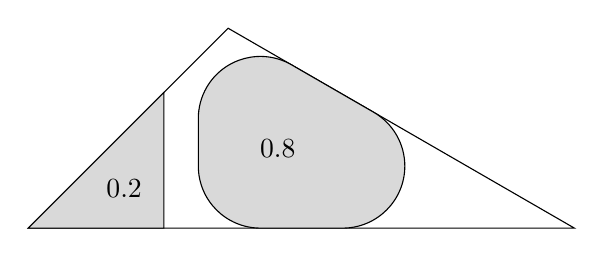
\begin{tikzpicture}[scale=2]
        \hatsinhat{45}{30}{0.8}{0}
    \end{tikzpicture}
    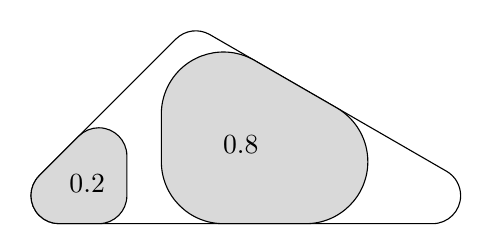
\begin{tikzpicture}[scale=2]
        \hatsinhat{45}{30}{0.8}{0.1}
    \end{tikzpicture}

    \caption{Rounding all hats' corners by the same radius does not affect the packing.}
    \label{fig:rounding-hats}
\end{figure}

\chapter{Triangles}

\begin{theorem}
    For any obtuse or right triangle with an incircle of area $a$, for any $b > a$ there are instances in $\C(b)$ which cannot be packed into the triangle.
\end{theorem}

\begin{proof}
    The instance $\{b\}$ cannot be packed, as the incircle is by definition the largest circle which fits into the triangle.
\end{proof}

\begin{theorem}
    An obtuse or right triangle with an incircle of area $a$ is an $a$-shape.
\end{theorem}

\begin{proof}
    The triangle is an $(a,0)$-hats, which is an $a$-shape.
\end{proof}

%\begin{theorem}
%    Each $A \in \C(a)$ can be packed into an isosceles triangle with a largest angle $\gamma$ between $\frac{\pi}{2}$ and $\frac{\pi}{3}$ and an area of $a\frac{1+\frac{1}{\sin(\gamma)}}{\pi}$.
%\end{theorem}
%
%\begin{theorem}
%    For any $0 < x$ and $0 < y$, there are always 
%    a $(x+z)$-hat and a
%    Each $A \in \C(a)$ can be packed into an obtuse triangle with an incircle of area $a$.
%\end{theorem}
%
%\chapter{Squares}
%
%\begin{figure}[htb]
%    \centering
%
%    \begin{tikzpicture}[scale=2]
%        \hatsinsquare{0.5}
%    \end{tikzpicture}
%    \begin{tikzpicture}[scale=2]
%        \hatsinsquare{0.49}
%    \end{tikzpicture}
%    \begin{tikzpicture}[scale=2]
%        \hatsinsquare{0.4}
%    \end{tikzpicture}
%    \begin{tikzpicture}[scale=2]
%        \hatsinsquare{0.2}
%    \end{tikzpicture}
%    \begin{tikzpicture}[scale=2]
%        \hatsinsquare{0}
%    \end{tikzpicture}
%
%    \caption{Hat-in-square packings for different values of $\frac{x}{x+y}$}
%    \label{fig:hatsinsquare}
%\end{figure}
%
%\begin{theorem}\label{th:hatsinsquare}
%    For any $0 \le x \le y$, an $x$-hat and a $(y,y-x)$-hat can always be packed into a square with an area of $\Psi(x+y)$.
%\end{theorem}
%
%\begin{proof}
%    Place the tips of the hats in two opposing corners of the square, like in \Cref{fig:hatsinsquare}.
%    This placement constitues a valid packing if (1) the hats fit into the square individually and (2) the hats do not overlap.
%
%    \begin{itemize}
%        \item[(1)]
%            The hats fit into the square individually if their diagonal never gets larger than the square's edge length $\sqrt{\Psi(x+y)} = \frac{1+\s}{\sqrt{\pi}}\sqrt{x+y}$.
%            As $x \le \frac {x+y} 2$, \Cref{lm:sizes} directly tells us that the $x$-hat has a diagonal of at most
%            \begin{align*}
%                d(x,0) \le d(\frac{x+y}{2},0) = \sqrt{\frac{\frac{x+y}{2}}{\pi}}(2+\s) + 0 = \sqrt{\Psi(x+y)}
%            \end{align*}
%
%            As for the $(y,y-x)$-hat, its diagonal is also never larger than $\sqrt{\Psi(x+y)}$: \todo[inline]{algebraic proof TBD :-)}
%
%            \begin{tikzpicture}
%                \begin{axis}[height=5cm,xtick={0,0.5},xlabel=$\frac{x}{x+y}$,domain=0:0.5,legend pos=outer north east,no markers,samples=500]
%                    \addplot[red,thick] {sqrt((1-x)/pi)*(2+sqrt(2))-sqrt((1-2*x)/pi)*sqrt(2)};
%                    \addplot[blue,thick] {(1+sqrt(2))/sqrt(pi)};
%                    \legend{$\frac{d{(y,y-x)}}{\sqrt{x+y}}$,$\sqrt{\Psi}$}
%                \end{axis} 
%            \end{tikzpicture}
%
%            %\begin{align*}
%            %    d(y,y-x)
%            %    &= \sqrt{\frac{y}{\pi}}(2+\s)-\sqrt{\frac{y-x}{\pi}}\s\\
%            %    &\le \sqrt{\frac{\frac{x+y}{2}}{\pi}}(2+\s)-\sqrt{\frac{y-y}{\pi}}\s\\
%            %    &= \frac{1+\s}{\sqrt{\pi}}\sqrt{x+y} = \sqrt{\Psi(x+y)}
%            %\end{align*}
%
%        \item[(2)]
%            The hats don't overlap if their combined height never exceeds $\sqrt{2\Psi(x+y)}$, the square's diagonal:
%            \begin{align*}
%                h(x) + h(y)
%                &= \sqrt{\frac{x}{\pi}}(1+\s) + \sqrt{\frac{y}{\pi}}(1+\s)\\
%                &= \frac{1+\s}{\sqrt\pi}(\sqrt{x}+\sqrt{y})\\
%                &\le \frac{1+\s}{\sqrt\pi}(\sqrt{2x+2y})\\
%                &= \s\frac{1+\s}{\sqrt\pi}\sqrt{x+y} = \sqrt{2\Psi(x+y)} \qedhere
%            \end{align*}
%    \end{itemize}
%\end{proof}
%
%
%Finally, we can bring the \textsc{Split} algorithm and the properties of the hat shapes together and give constructive proofs for the existence of circle packings:

\begin{theorem}\label{th:circlesinhat}
    Each right $(a,b)$-hat is an $(a,b)$-shape.
\end{theorem}

\begin{proof}
    Call the hat's smaller angles $\alpha$ and $\beta$. Set $f = $
%    If $A$ only consists of a single $a$-circle, it is the incircle of the $(a,b)$-hat, so it can be packed. Otherwise, by \Cref{th:split-property}, \textsc{Split} decomposes $A$ into $X \in \C(x)$ and $Y \in \C(y,y-x)$. As all circles in $A$ are at least of area $b$, the same is true for $X$ and $Y$, so $X \in \C(x,b)$ and $Y \in \C(y,\max(y-x,b))$
%    If we assume this theorem to be true for all instances with fewer circles than $A$, we can pack $X$ into a $(x,b)$-hat and $Y$ into a $(y,\max(y-x,b))$-hat. By \Cref{th:roundedhatsinhat}, we can pack those two hats into the $(a,b)$-hat.
\end{proof}
%
%We are now ready to prove our main theorem:
%
%\begin{theorem}\label{th:circlesinsquare}
%    Each $A \in \C(a)$ can be packed into a square with an area of $\Psi a$.
%\end{theorem}
%
%\begin{proof}
%    If $A$ only consists of a single $a$-circle, it can be placed at the center of the square, as its diameter of $2\sqrt{\frac{a}{\pi}} \approx 1.12838\sqrt{a}$ is smaller than the squares edge length $\sqrt{\Psi a} \approx 1.36207\sqrt{a}$. Otherwise, by \Cref{th:split-property}, \textsc{Split} decomposes $A$ into $X \in \C(x)$ and $Y \in \C(y,y-x)$. By \Cref{th:circlesinhat}, we can pack $X$ into a $x$-hat and $Y$ into a $(y,y-x)$-hat. By \Cref{th:hatsinsquare}, we can pack those two hats into the square.
%
%    See \Cref{fig:example} for a complete example packing.
%\end{proof}
%
%\begin{figure}[htb]
%    \centering
%    \includegraphics[width=0.5\textwidth]{square_example.png}
%    \caption{Packing of an example instance.}
%    \label{fig:example}
%\end{figure}
%
%\chapter{Conclusions and Future Work}
%
%\appendix

\end{document}
